\documentclass[a4paper,10pt]{article}

% Language.
\usepackage[english]{babel}

% Math packages.
\usepackage{amssymb}
\usepackage{amstext}
\usepackage{amsmath}

% Smaller margins.
%\usepackage[margin=0.5in]{geometry}

% Graphic package.
\usepackage{graphicx}

% Monospace font.
\usepackage{inconsolata}

\begin{document}

%%%%%%%%%%%%%%%%%%%%%%%%%%%%%%%%%%%%%%%%%%%%%%%%%%%%%%%%%%%%%%%%%%%%%%%%%%%%%%%
% System Architecture
%%%%%%%%%%%%%%%%%%%%%%%%%%%%%%%%%%%%%%%%%%%%%%%%%%%%%%%%%%%%%%%%%%%%%%%%%%%%%%%
\section{System Architecture}
\label{sec:system-architecture}
% Technical description of the system.
In the following section we will give an overview of the architecture of the system and the individual components.
The components are divided into three categories, namely hardware components, software components and the interaction between hardware and software components.

	%%%%%%%%%%%%%%%%%%%%%%%%%%%%%%%%%%%%%%%%%%%%%%%%%%%%%%%%%%%%%%%%%%%%%%%%%%%
	\subsection{Hardware Components}
	% Nice image here.
	\subsubsection{Tabletop}
	The tabletop consists of a table where we replaced the table top with a glass plate with a layer of tracing paper on top.
	Underneath the glass plate a huge mirror is placed that reflects the projects image by the beamer. 
	Besides the mirror there is a small webcam that records everything that happens on the screen and everything that is visible through the tracing paper. 

	\begin{figure}[h!]
	\caption{The tabletop}
	\centering
	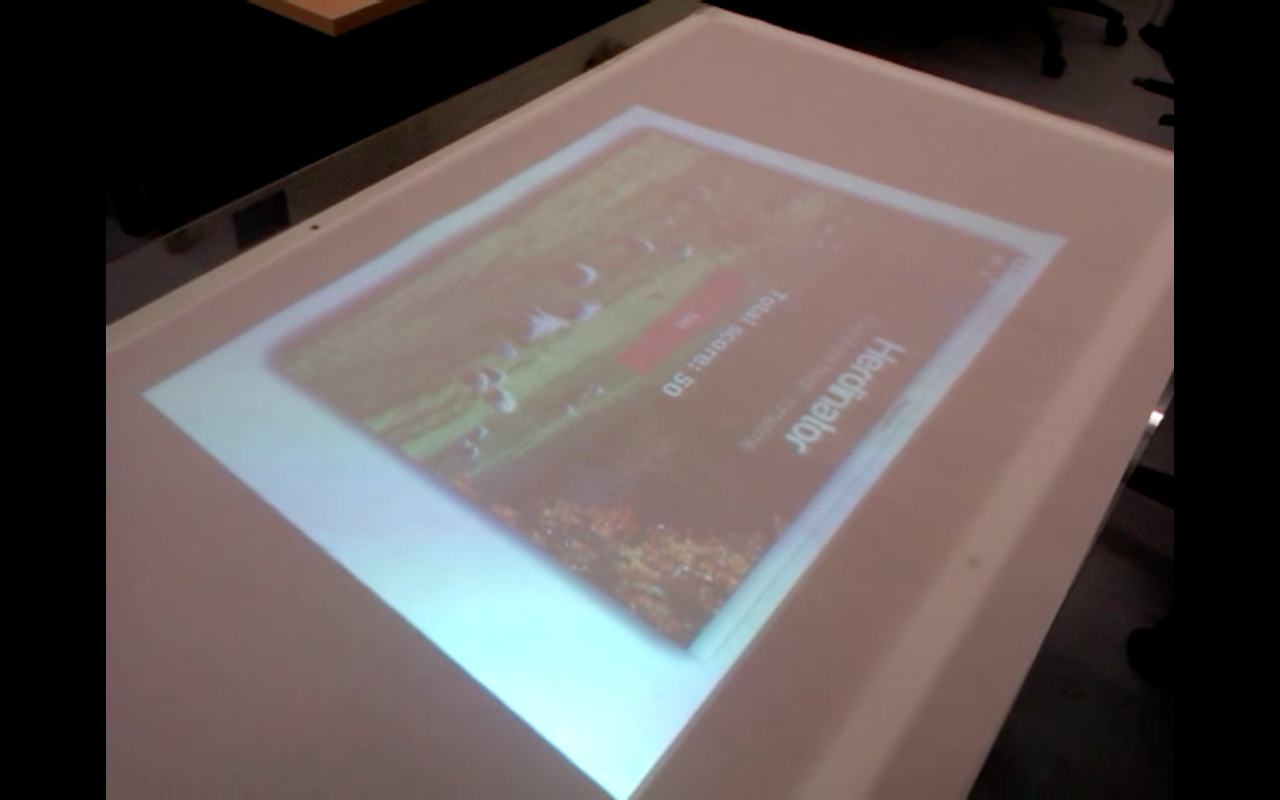
\includegraphics[width=0.5\textwidth]{images/tabletop}
	\end{figure}

	\subsubsection{Beamer}
	The beamer that projects an image on the tabletop is borrowed from our department and is a small portable beamer.
	The image that is projected is sharp enough for the user to get an accurate idea of what is happening on the screen. 
	As the projected image is not projected very wide the mirror in the tabletop is used. 

	\begin{figure}[h!]
	\caption{The tabletop}
	\centering
	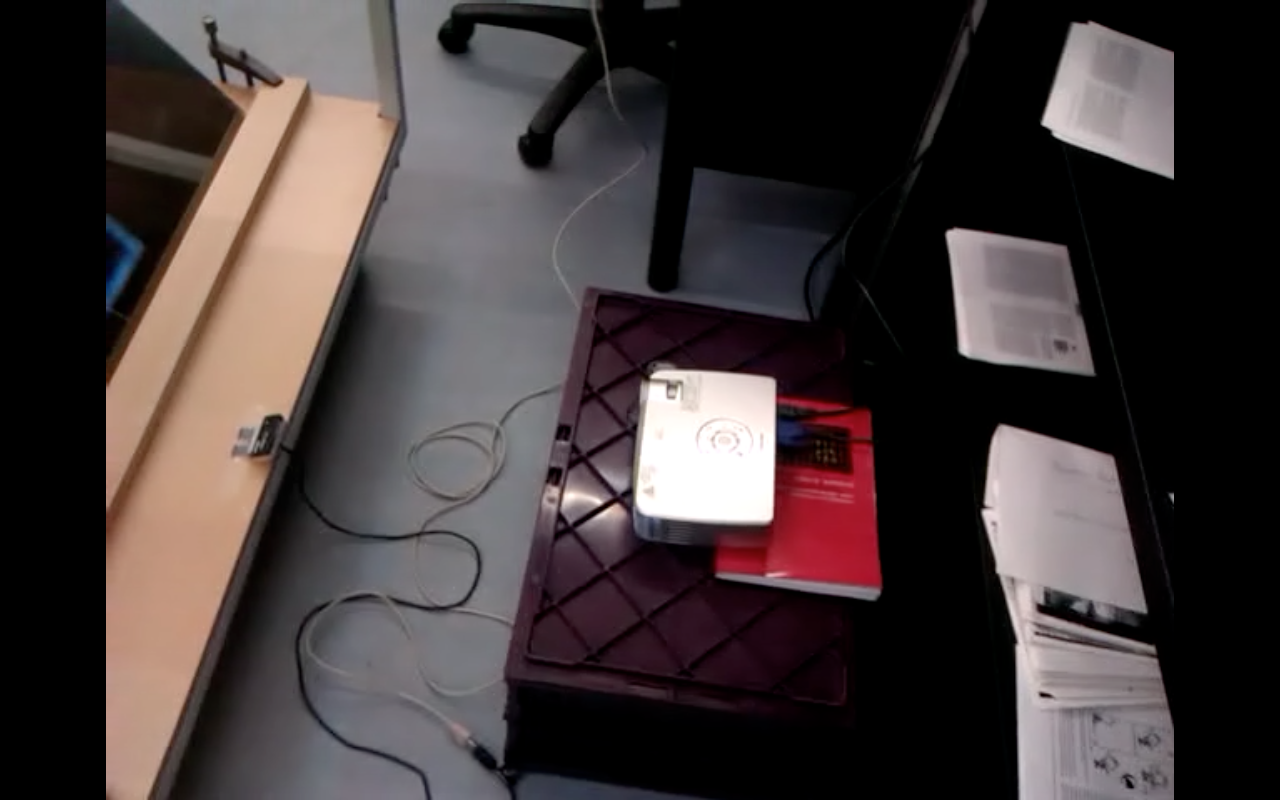
\includegraphics[width=0.5\textwidth]{images/beamer}
	\end{figure}

	\subsubsection{Webcam}
	The webcam used for our project is a simple consumer Microsoft Livecam. 
	Our webcam records in a medium quality high enough for our simple application. 
	Of course, using a better webcam would have improved our application but our current results were already acceptable. 

	\begin{figure}[h!]
	\caption{The webcam}
	\centering
	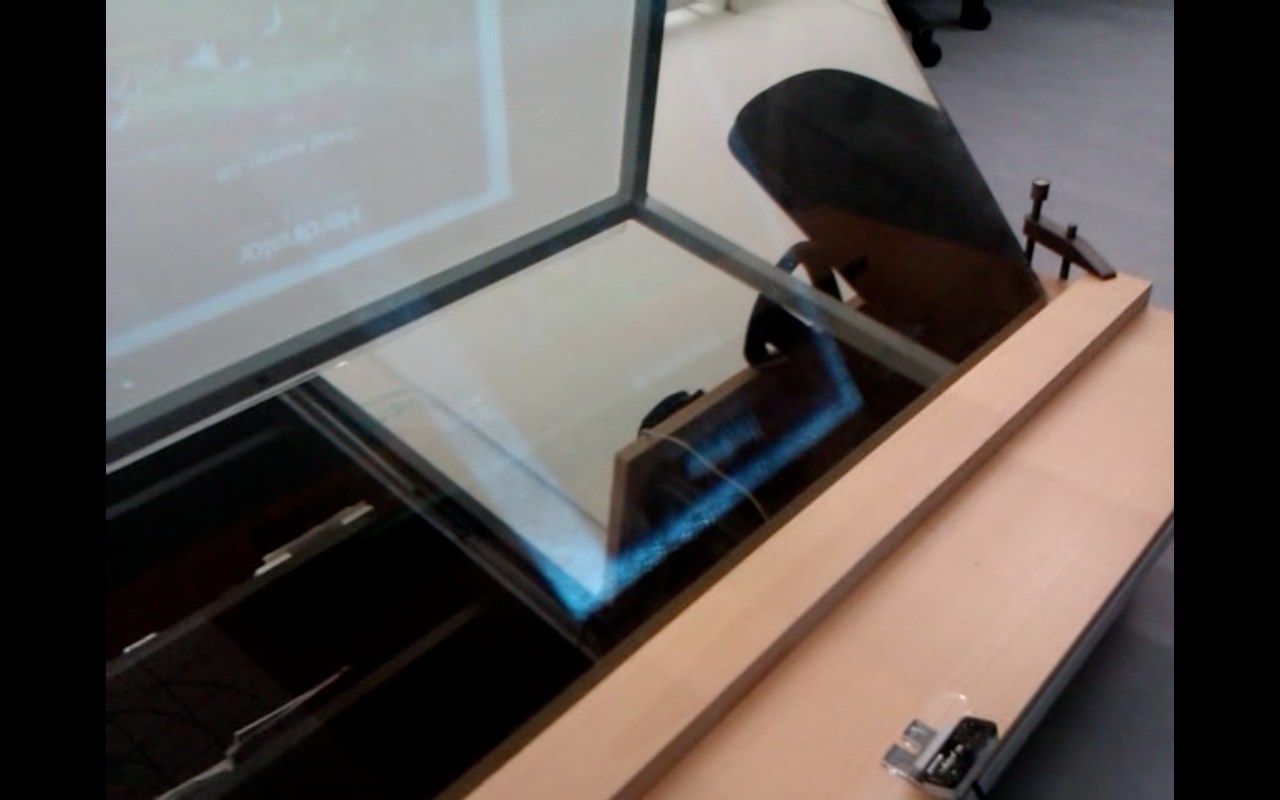
\includegraphics[width=0.5\textwidth]{images/webcam}
	\end{figure}

	%%%%%%%%%%%%%%%%%%%%%%%%%%%%%%%%%%%%%%%%%%%%%%%%%%%%%%%%%%%%%%%%%%%%%%%%%%%
	\subsection{Software Components}
	\label{sec:software-components}
	In the following section an overview is given of the individual software components, namely the \emph{game}, the \emph{server} and the \emph{Android application}.
	In section~\ref{sec:communication-protocol} an overview is given on how the server and the Android application communicate with each other.
	% Even nicer images here.

		%%%%%%%%%%%%%%%%%%%%%%%%%%%%%%%%%%%%%%%%%%%%%%%%%%%%%%%%%%%%%%%%%%%%%%%%%
		\subsubsection{Game}
		The game itself is written in Java and is built using the open source game platform Slick2D \cite{Slick2D}.
		Slick2D is primarily a wrapper around LWJGL \cite{LWJGL} and provides certain functionality to make it easier to develop games.
		LWJGL is primarily intended to allow developers easy access to certain libraries, like OpenGL, OpenCL, OpenAL, etc., to be used effectively and efficiently in Java.
		On itself LWJGL is not very suited to develop games with, however Slick2D adds extra functionality on top of LWJGL, like a game loop, a state switching mechanism, animations, etc.
		
		The game itself is divided into several parts, each containing many different objects of which most are not very important nor interesting to discuss.
		Therefor we will only discuss the core parts, which are the different states, the \emph{GameManager}-object and the \emph{Map}-object to to get reasonable overview of the game.
		
		\paragraph{States}
		A small, but useful, feature of Slick2D is that it contains a state switching mechanism.
		This allowed us to create several states from which you can switch to any state.
		In figure~\ref{fig:game-state-diagram} an overview is given of the different states and in what way one can switch to another state through the normal usage of the game.
		The game starts in the \emph{LoadingState} after which it automatically transition to the \emph{ModalitySelectorMenuState}.
		In this state the user is able to select, via buttons on the screen, which modality it wants to use to play the game with.
		If the mouse/touch modality is chosen the game will transition to the \emph{ModalityMouseAndTouchMenuState}.
		If the tangible modality is chosen the game will transition to the \emph{ModalityTangiblesMenuState}.
		In both states the user is either able to go back or start the game after the appropriate preparations have been made.
		In the \emph{GameState} the actual game is run.
		If one of the two ending conditions, namely herding all the sheep or no more time left, has been reached the game will transition to the \emph{GameScoreMenuState}.
		In this state the user is presented with the score and given the only possibility to exit the game.
		There used to be the possibility of going back to the \emph{ModalitySelectorMenuState}, however there were some issues in resetting the game properly, thus we have removed this feature.
		
		\begin{figure}
			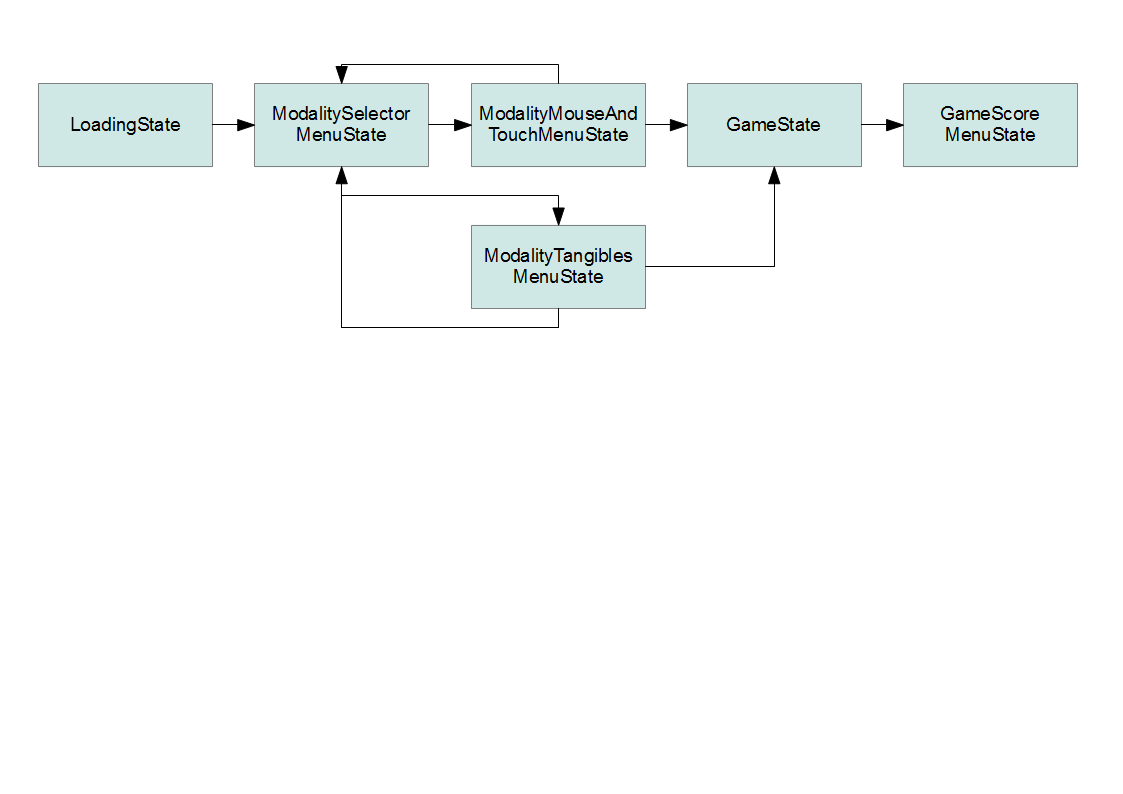
\includegraphics[width=\columnwidth]{images/game-state-diagram.png}
			\caption{Overview of the different states in the game.}
			\label{fig:game-state-diagram}
		\end{figure}
		
		\paragraph{GameManager}
		With the state switching mechanism of Slick2D it is not possible to transfer information between different states.
		Furthermore it is very practical to have a global object which can hold global information such that it is not necessary for each class to hold 
		Therefor we have created the \emph{GameManager}-object.
		\emph{GameManager} is a global singleton-object, meaning only a single instance of the object is available.
		Each object of the game can read and write specific information from and to the \emph{GameManager}.
		For example, \emph{GameManager} holds information about the current map being played and which players are currently playing the game.		
		
		\paragraph{Map}
		Arguably the most important object of the game is the \emph{Map}-object.
		\emph{Map} is primarily a container-object, holding many other objects, like sheep, dogs, cookies, etc.
		Furthermore it also contains functionality with which it is possible to perform correct moving and pathfinding behavior.
		Since \emph{Map} is one of the objects many other objects need to be aware of, it is also available through \emph{GameManager}.		
		
		%%%%%%%%%%%%%%%%%%%%%%%%%%%%%%%%%%%%%%%%%%%%%%%%%%%%%%%%%%%%%%%%%%%%%%%%%
		\subsubsection{Server}
		The server has a key role in our setup.
		It handles the communication between the Android application and the game.
		For the server a portable version of Tomcat was used which is started at runtime every time the game starts.
		On the server we ran a single servlet which would handle all the communication between the server and the Android application.
		This setup is very flexible, since no one has to have Tomcat installed and configured on their system.
		Furthermore it allows for a tight coupling between the game and the server application.
		On the one hand a tight coupling can be seen as a disadvantage since it becomes difficult to separate the server from the game.
		On the other hand it also saves a lot of time trying to built a suitable interface between the server and the game.
				
		Since the server is tightly couple with the game it is able to access all the components of the game through \emph{GameManager}.
		Using \emph{GameManager} the server is able to add and remove players which connect respectively disconnect themselves.
		@TODO: ... 
		
		\subsubsection{Android Application}
		In our experiment the Android application with the mobile phone is used as a tangible object.
		The Android application is used to communicate with the game via commands send to the server.
		The Android application consists of three screens, namely a \emph{login}-screen~\ref{fig:android-application-screen1}, a \emph{select object}-screen~\ref{fig:android-application-screen2} and a \emph{use selected object}-screen~\ref{fig:android-application-screen3}.
		In the \emph{login}-screen the user has to fill in the details of the server and the mark id which is on the back of the mobile phone.
		If the Android application is able to successfully connect to the server it switches to the \emph{select object}-screen.
		In the \emph{select object}-screen the user is able to select which object it wants to use.
		In our case there are only two objects to choose from, namely a whistle and a cookie.
		Once the user has selected an object the Android application switches to the \emph{use selected object}-screen.
		In the \emph{use selected object}-screen the user is able to use the object, by pressing it.
		If the object is used and the mobile phone is placed on the interactive table it will be registered by the game and actors can act accordingly.
		If the user wants to select a different object it can perform a horizontal backwards swipe to return to the \emph{select object}-screen.
		
		\begin{figure}[ht]
			\begin{minipage}[b]{0.30\linewidth}
				\centering
				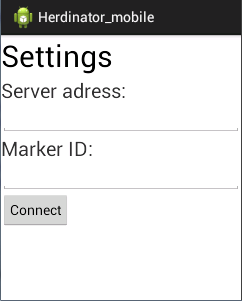
\includegraphics[width=\textwidth]{android-application-screen1.png}
				\caption{\emph{Login}-screen}
				\label{fig:android-applications-sreen1}
			\end{minipage}
			\hspace{0.1cm}
			\begin{minipage}[b]{0.30\linewidth}
				\centering
				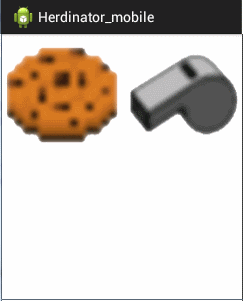
\includegraphics[width=\textwidth]{android-application-screen2.png}
				\caption{\emph{Select object}-screen}
				\label{fig:android-application-screen2}
			\end{minipage}
			\hspace{0.1cm}
			\begin{minipage}[b]{0.30\linewidth}
				\centering
				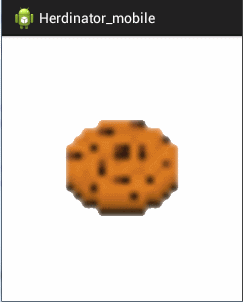
\includegraphics[width=\textwidth]{android-application-screen3.png}
				\caption{\emph{Use selected object}-screen}
				\label{fig:android-application-screen3}
			\end{minipage}
		\end{figure}
		
	%%%%%%%%%%%%%%%%%%%%%%%%%%%%%%%%%%%%%%%%%%%%%%%%%%%%%%%%%%%%%%%%%%%%%%%%%%%	
	\subsection{Interaction Between Hardware and Software Components}
	% Using the title 'Interaction Between Hardware and Software Components' (or something similar) is more consistent with the rest.
	% So first you could give an overview of the different components needed for this and then how it is all tied together.

	\subsubsection{reacTIVision}
	\label{sec:reactivision}
	reactTIVision is a software component that is able to detect both finger touches on a screen and specific markers. 
	The source image (taken from the webcam under the table) is first converted to a black and white image with an adaptive thresholding algoritm. 
	This image is converted into black and white regions, which is searched for unique sequences encoded into the fiducial symbols. \cite{reactivision}.
	At every frame it detects what markers are present and sends the corresponding event as described in section \ref{sec:tuioprotocol}

	\subsubsection{Community Core Vision}
	\label{sec:communitycorevision}	
			Community Core Vision (CCV) is a computer vision program that takes our video input stream (taken from the webcam under the table) and outputs tracking data. \cite{ccv}.
		    	Several features of CCV include several filters, input and output switchers and a calibration mode. 
			Using image processing CCV checks for the blobs that represent the tops of the fingers of the user. 
			The locations and ID's of these blobs are send using the TUIO protocol described in section \ref{sec:tuioprotocol}.
			\begin{figure}[h!]
			  \caption{The game}
			  \centering
			  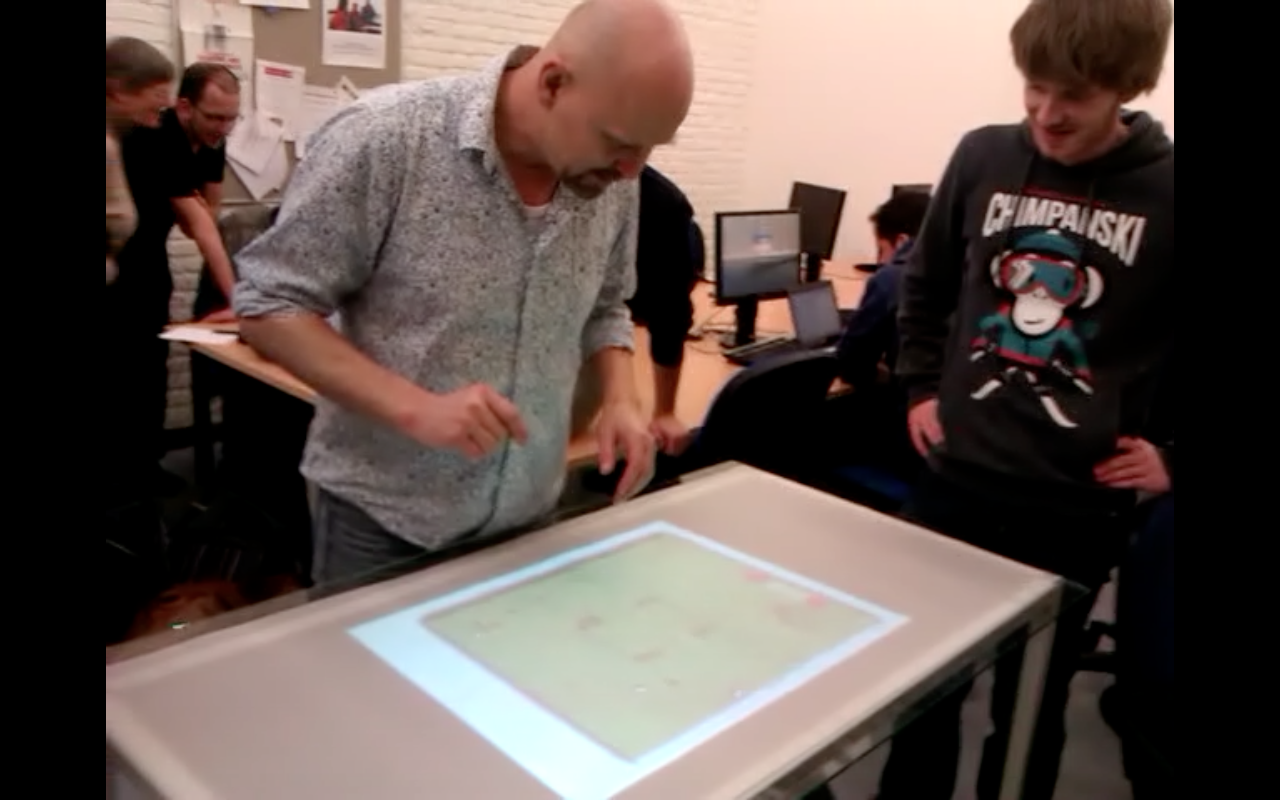
\includegraphics[width=0.5\textwidth]{images/tafelgebruik}
			\end{figure}
		
			\subsubsection{TUIO Protocol}
			\label{sec:tuioprotocol}
			The TUIO Protocol consists of a series of event-based communication using OSC messages over port 3333. \cite{tuioProtocol}. 
			Using a JAVA library our program catches these messages and calls an event every time a:
			\begin{enumerate}
				\item finger is added to the screen
				\item finger is removed from the screen
				\item finger moved on the screen
				\item marker is added to the screen
				\item marker is removed from the screen
				\item marker is moved on the screen
			\end{enumerate}
			These events also include a TUIOPoint object that contains among other the:
			\begin{enumerate}
				\item Location of the finger or marker
				\item ID of the finger or marker
			\end{enumerate}
			Using these events the objects in our game are updated to their locations respective to the game on the screen as described in section \ref{waar wordts dit uitgelegd?}.
		
%%%%%%%%%%%%%%%%%%%%%%%%%%%%%%%%%%%%%%%%%%%%%%%%%%%%%%%%%%%%%%%%%%%%%%%%%%%%%%%
% Communication Protocol
%%%%%%%%%%%%%%%%%%%%%%%%%%%%%%%%%%%%%%%%%%%%%%%%%%%%%%%%%%%%%%%%%%%%%%%%%%%%%%%		
\section{Communication Protocol}
\label{sec:communication-protocol}
In order for the server and the Android application to exchange information with each other we had to design a communication protocol.
The communication protocol is used by the Android application to execute certain commands to let the game "know" a certain action has to be performed.

The Android application exchange information through a request-response paradigm.
The Android application sends a specific HTTP request which is interpreted by the server after which the server responds with JSON-formatted messages.
In order to read and write the messages the JSON.simple~\cite{JSONsimple} library is used.
Since both the Android application and the server use the same JSON library to read and write the messages there would be no problems in exchanging them.
Using JSON-formatted messages has several advantages:
\begin{itemize}
	\item
		\textbf{Easy to read and write programmatically}:
		Even though in our case a library handles most of the work, other formats, like XML, require more effort to get working.
	\item
		\textbf{Easy to read}:
		JSON-formatted messages are clear and concise making it easy to understand en verify the messages by hand, which helps in debugging.
	\item
		\textbf{Easy to expand}:
		The current setup makes it easy to add extra information to the messages, for example an error message when the request is unsuccessful.
\end{itemize}

For each request-response the Android application initiates the communication by sending one of the predefined requests as can be found below.
The server handles the request and responds either successfully, of which the specification can be found below, or unsuccessfully.
The message for an unsuccessful response is simply: \texttt{\{success:false\}}.

\subsection{Commands}
Below a list of all the accepted requests is given.
In general a certain order is required in executing the request.
For example, first one has to execute the \emph{connect}-command before one can execute the \emph{select}-command and only after a successful \emph{select}-command one can execute the \emph{use}-command.
No specific overview of the possible orders in which they can be executed is given, since it should follow from the specification.
	
	\subsubsection{Connect}
	Request: \texttt{?action=connect\&markId=[INTEGER]} \\
	Returns: \texttt{\{success:true, phoneId:[INTEGER]\}} \\

	\noindent Using the \emph{connect}-command the Android application is able to connect itself with the server.
	The parameter \texttt{markId} is required and should contain the id which corresponds with the mark on the back of the phone.
	If the request is successful a unique identifier \texttt{phoneId} is returned which should be used for every other request made.

	\subsubsection{Disconnect}
	Request: \texttt{?action=disconnect\&phoneId=[INTEGER]} \\
	Returns: \texttt{\{success:true\}} \\

	\noindent Using the \emph{disconnect}-command the Android application is able to disconnect itself with the server.
	The parameter \texttt{phoneId} is required and denotes the unique identifier which is returned on a successful connect.
	After a successful request any subsequent request with the given \texttt{phoneId} will fail.

	\subsubsection{Select}
	Request: \texttt{?action=select\&phoneId=[INTEGER]\&item=[STRING]} \\
	Returns: \texttt{\{success:true\}} \\

	\noindent Using the \emph{select}-command the Android application is able to select an item.
	The parameter \texttt{phoneId} is required and denotes the unique identifier which is returned on a successful connect.
	The parameter \texttt{item} is required and denotes the item to be selected. The supported items are: \emph{whistle} and \emph{cookie}.

	\subsubsection{Use}
	Request: \texttt{?action=use\&phoneId=[INTEGER]} \\
	Returns: \texttt{\{success:true\}} \\

	\noindent Using the \emph{use}-command the Android application is able to use the selected item.
	The parameter \texttt{phoneId} is required and denotes the unique identifier which is returned on a successful connect.
	If an item is successfully selected using the \emph{select}-command the item will appear in the game, which makes it possible for actors to respond accordingly.

\bibliographystyle{apalike}
\bibliography{report}
\end{document}




%@misc{Slick2D,
%title={Slick2D},
%howpublished={\url{http://www.slick2d.org/}},
%note={Last accessed: 07-02-2013}
%}

%@misc{LWJGL,
%title={Lightweight Java Game Library (LWJGL)},
%howpublished={\url{http://www.lwjgl.org/}},
%note={Last accessed: 07-02-2013}
%}

%@misc{JSONsimple,
%title={JSON.simple},
%howpublished={\url{http://code.google.com/p/json-simple/}},
%note={Last accessed: 07-02-2013}
%}
